\section{Frekvensanalys}

\paragraph{Fundamental ide}
Eftersom periodiska funktioner kan skrivas som en summa av trigonometriska funktioner och funktioner som avtar tillräcklig snabbt kan skrivas som en integral över trigonometriska funktioner, vet vi att när vi studerar linjära system räcker det att studera systemets respons på en enda term, alltså en enda trigonometrisk funktion, och se hur den beror av frekvensen. Om vi tillför en signal $u = \sin{\omega t}$ till ett system med överförningsfunktion $G$ får vi
\begin{align*}
	y &= \integ{0}{\infty}{\tau}{g(\tau)u(t - \tau)} \\
	  &= \Im\left(\integ{0}{\infty}{\tau}{g(\tau)e^{i\omega(t - \tau)}}\right) \\
	  &= \Im\left(e^{i\omega t}\integ{0}{\infty}{\tau}{g(\tau)e^{-i\omega\tau}}\right) \\
	  &= \Im(e^{i\omega t}G(i\omega)) \\
	  &= \abs{G(i\omega)}\sin(\omega t + \arg{G(i\omega)}).
\end{align*}
Det kan även finnas transienta termer här, men om systemet är stabilt kommer dessa försvinna över tid. Vi ser alltså att systemets svar beror av $G(i\omega)$.

\paragraph{Nyquistdiagram}
Ett Nyquistdiagram är en uppritning av $G(i\omega)$ för $0 < \omega < \infty$. Vi kan se att detta i stort sett är den intressanta delen av Nyquistkurvan.

\paragraph{Bodediagram}
Ett Bodediagram är en diagram av $\abs{G(i\omega)}$ och $\arg{G(i\omega)}$ som funktioner av $\omega$.

\paragraph{Skärfrekvens}
Skärfrekvensen $\omega_{\text{c}}$ är frekvensen för vilken Nyquistkurvan skär enhetscirkeln. Det är en tummregel att denna är proportionell mot systemets bandbredd, som vi kommer diskutera sedan.

\paragraph{Fasmarginal}
Fasmarginalen $\phi_{\text{m}}$ är vinkeln mellan negativa $x$-axeln och punkten där Nyquistkurvan skär enhetscirkeln. Mer specifikt kan vi skriva $\phi_{\text{m}} = \pi + \arg{G(i\omega_{\text{c}})}$.

\paragraph{Fasskärfrekvens}
Fasskärfrekvensen $\omega_{\text{p}}$ är frekvensen så att $\arg{G_{\text{O}}(i\omega_{\text{p}})} = -\pi$.

\paragraph{Amplitudmarginal}
Amplitudmarginalen ges av $A_{\text{m}} = \frac{1}{\abs{G_{\text{O}}(i\omega_{\text{p}})}}$.

\paragraph{Alternativt förenklad Nyquist-kriterium}
Det förenklade Nyquistkriteriet kan nu formuleras som $\phi_{\text{m}} > 0,\ A_{\text{m}} > 1$.

\paragraph{Bandbredd}
Bandbredden är bredden på det frekvensintervallet där $\abs{G(i\omega)} \geq \frac{1}{\sqrt{2}}$ i relativa enheter, vilket motsvarar förstärkning större än \SI{3}{\decibel}, och benämnas $\omega_{\text{B}}$. Bandbredden kan ge information om systemets tillväxt, då hög bandbredd typiskt betyder snabb tillväxt.

\paragraph{Resonansfrekvens}
Resonansfrekvensen $\omega_{\text{r}}$ är den frekvens som ger starkast respons i systemet.

\paragraph{Resonanstopp}
Resonanstoppen är $M_{\text{p}} = \abs{G(i\omega_{\text{r}})}$ i relativa enheter (?), och ger typiskt en indikation på hur mycket översläng man får. Man önskar typiskt att denna ska vara liten.

\paragraph{Dekomponering av Bodediagram}
Vi skriver överförningsfunktionen som
\begin{align*}
	G(i\omega) = \frac{K}{s^{p}}\frac{\prod\left(1 +\frac{i\omega}{z_{i}}\right)}{\prod\left(1 +\frac{i\omega}{p_{i}}\right)},
\end{align*}
som har poler i $-z_{i}$ och nollställen i $-p_{i}$. En sådan överförningsfunktion ger
\begin{align*}
	\log{\abs{G(i\omega)}} = \log{K} + \sum\log{\abs{1 +\frac{i\omega}{z_{i}}}} - \sum\log{\abs{1 +\frac{i\omega}{p_{i}}}},\ \arg{G(i\omega)} = -p\frac{\pi}{2} + \sum\arctan{\frac{\omega}{z_{i}}} - \sum\arctan{\frac{\omega}{p_{i}}}.
\end{align*}
Alltså är Bodeplottet en summa av bidrag från enstaka faktorer, eventuellt två komplexkonjugerade parade ihop. Vi studerar de därför var för sig.

\paragraph{Bodediagram för en potens}
Betrakta en faktor $s^{p}$ i överförningsfunktionen. För den gäller att
\begin{align*}
	\log{\abs{G(i\omega)}} = p\log{\omega},\ \arg{G(i\omega)} = -p\frac{\pi}{2}.
\end{align*}
Detta motsvarar en rät linje med lutning $p$ i Bodediagrammet och en konstant fassänkning.

\paragraph{Bodediagram för en linjär faktor}
En enda faktor $1 +\frac{i\omega}{z_{i}}$, under antagandet att $z_{i}$ är reell, har
\begin{align*}
	\log{\abs{G(i\omega)}} = \frac{1}{2}\log(1 + \frac{\omega^{2}}{z_{i}^{2}})\ \arg{G(i\omega)} = \arctan{\frac{\omega}{z_{i}}}.
\end{align*}
Lågfrekvensasymptoten är $0$, medan högfrekvensasymptoten är $\log{\frac{\omega}{z_{i}}}$, alltså en rät linje med lutning $1$ i en log-log-plot. Dessa två asymptoterna skär varandra för $\omega = z_{i}$. I denna punkten ändrar bodeplotten brått sin lutning. Denna punkten kallas då bodeplottens brytpunkt.

\paragraph{Bodediagram för ett polynom av andra ordningen}
Betrakta två faktorer
\begin{align*}
	\left(1 +\frac{i\omega}{z_{i}}\right)\left(1 +\frac{i\omega}{z_{i}^{*}}\right) = 1 - \frac{\omega^{2}}{\abs{z_{i}}^{2}} + 2i\omega\left(\frac{1}{z_{i}} + \frac{1}{z_{i}^{*}}\right) = 1 - \frac{\omega^{2}}{\abs{z_{i}}^{2}} + 2i\frac{\omega}{\abs{z_{i}}^{2}}(z_{i} + z_{i}^{*}) = 1 - \frac{\omega^{2}}{\abs{z_{i}}^{2}} + 2i\frac{\omega}{\abs{z_{i}}}\cos{\arg{z_{i}}}.
\end{align*}
Analogt med vad vi har gjort tidigare definierar vi $\abs{z_{i}} = \omega_{0},\ \zeta = \cos{\arg{z_{i}}}$. Vi har då
\begin{align*}
\log{\abs{G(i\omega)}} = \frac{1}{2}\log(\left(1 - \frac{\omega^{2}}{\omega_{0}^{2}}\right)^{2} + 4\frac{\omega^{2}}{\omega_{0}^{2}}\zeta^{2}),\ \arg{G(i\omega)} = \arctan{\frac{2\frac{\omega}{\omega_{0}}\zeta}{1 - \frac{\omega^{2}}{\omega_{0}^{2}}}}.
\end{align*}
Lågfrekvensasymptoten är $0$. Högfrekvensasymptoten är $2\log{\frac{\omega}{\omega_{0}}}$, vilket är en rak linje med lutning $2$ i en log-log-plot. Nära $\omega = \omega_{0}$ försvinner den kvadratiska termen, och Bodediagrammet beter sig som $\log{\frac{\omega}{\omega_{0}}}$, alltså en rak linje med lutning $1$ i en log-log-plot. Denna asymptoten skär alla andra precis när $\omega = \omega_{0}$, varför detta är en dubbel brytpunkt för Bodediagrammet.

\paragraph{Ritning av Bodeplottar}
För att rita amplituddelen av ett Bodediagram, gör följande:
\begin{itemize}
	\item Faktorisera täljare och nämnare och identifiera poler och nollställen.
	\item Identifiera exponenten $p$.
	\item Identifiera $K$.
	\item Starta Bodediagrammet i $\log{K}$ och fortsätt i en rak linje med lutning $-p$.
	\item När du kommer till en reell pol, sänk lutningen med $1$.
	\item När du kommer till beloppet av ett par av komplexa poler, sänk lutningen med $2$.
	\item Gör samma för nollställena, men höj lutningen i stället.
\end{itemize}

\paragraph{Bodes relation}
Låt $G$ vara minimumsfas, dvs. ha alla sina nollställen och poler i vänstre halvplan, och $G(0) > 0$. Då gäller att om $\abs{G(i\omega)}$ i ett visst frekvensområde avtar med \SI{20}{\decibel} per dekad (en dekad är en ökning i frekvens med en faktor $10$), är $\arg{G(i\omega)}\approx \SI{-90}{\degree}$, och om $\abs{G(i\omega)}$ avtar med \SI{40}{\decibel} per dekad, är $\arg{G(i\omega)}\approx \SI{-180}{\degree}$.

\paragraph{Snabbhet och svängighet}
Vi kan med tidigare resultat se att om $G_{\text{O}}(i\omega)$ är nära $1$ blir $G_{\text{C}}(i\omega)$ stor, och om $G_{\text{O}}(i\omega)$ är liten blir även $G_{\text{C}}(i\omega)$ liten. Vi kan också se att ett ekvivalent kriterium för bandbredden är $\abs{G_{\text{O}}(i\omega) - 1} \leq \sqrt{2}$ för $\omega \geq \omega_{\text{B}}$.

\paragraph{Resonanstopp och fasmarginal}
Vi har
\begin{align*}
	M_{\text{p}} \geq \abs{G(i\omega_{\text{c}})} = \frac{1}{2\sin(\frac{1}{2}\phi_{\text{m}})}.
\end{align*}
Speciellt ger liten fasmarginal stort översläng.

\paragraph{Frekvensanalys av känslighetsfunktionen}
Betrakta ett system som i figur \ref{fig:negative_feedback_equiv}.
\begin{figure}[!ht]
	\centering
	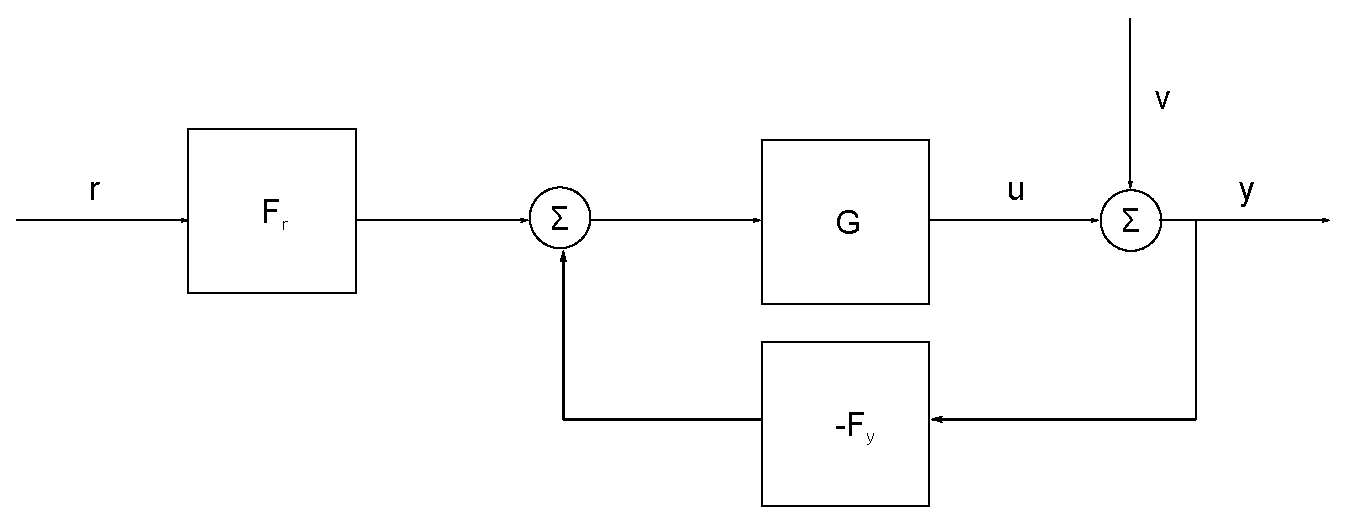
\includegraphics[width = \textwidth]{./Images/negative_feedback_equiv.eps}
	\caption{Illustration av tänkt reglersystem.}
	\label{fig:negative_feedback_equiv}
\end{figure}
Om $F_{r} = F_{y} = F$, skulle systemet vara ekvivalent med det välkända negativt återkopplade systemet. Vi är nu intresserade av att studera systemets känslighet för störningen.

Vi har allmänt
\begin{align*}
	Y = V + U = V + G(RF_{r} - YF_{y}),\ Y = \frac{GF_{r}}{1 + GF_{y}}R + \frac{1}{1 + GF_{y}}V,
\end{align*}
och känslighetsfunktionen ges då av
\begin{align*}
	S = \frac{1}{1 + GF_{y}}.
\end{align*}

Vi har
\begin{align*}
	\abs{S(i\omega)} = \abs{\frac{1}{1 + G(i\omega)F_{y}(i\omega)}} \leq M_{\text{s}},
\end{align*}
vilket kan skrivas som
\begin{align*}
	\abs{G(i\omega)F_{y}(i\omega) - (-1)} \leq \frac{1}{M_{\text{s}}}.
\end{align*}
Alltså måste Nyquistkurvan för $GF_{y}$ vara utanför en cirkel med mittpukt i $-1$ och radie $\frac{1}{M_{\text{s}}}$.

\paragraph{Robusthet}
Medan en modell kan ha en överförningsfunktion $G$, kan ett reellt system ha en överförningsfunktion $G' = G(1 + \Delta G)$, där $\Delta G$ är det relativa felet i överförningsfunktionen. Om man återkopplar systemet får man då
\begin{align*}
	Y' &= \frac{G'F}{1 + G'F}R \\
	   &= \frac{G'F(1 + GF)}{(1 + GF)(1 + G'F)}R \\
	   &= \frac{GF(1 + \Delta G)(1 + GF)}{(1 + GF)(1 + G'F)}R \\
	   &= \frac{GF(1 + \Delta G + GF + \Delta GGF)}{(1 + GF)(1 + G'F)}R \\
	   &= \frac{GF\Delta G + FG(1 + GF + \Delta GGF)}{(1 + GF)(1 + G'F)}R \\
	   &= \frac{GF\Delta G + FG(1 + G'F)}{(1 + GF)(1 + G'F)}R \\
	   &= \left(\frac{GF\Delta G}{(1 + GF)(1 + G'F)} + \frac{FG}{1 + GF}\right)R.
\end{align*}
Om återkopplingen är $U = FE$ fås
\begin{align*}
	Y' &= \frac{FG}{1 + GF}R + \frac{GF\Delta G}{(1 + GF)(1 + G'F)}R \\
	   &= (1 + S'\Delta G)Y,
\end{align*}
där $S'$ är känslighetsfunktionen för det verkliga systemet. Det relativa felet i $Y$ blir alltså $S'\Delta G$ blir det relativa felet i $Y$. Detta betyder att om systemets känslighetsfunktion är liten, får modellfel liten inverkan.

\paragraph{Robusthetskriteriet}
Antag att $G$ ger ett system som är stabilt. Är då ett motsvarande verkligt system stabilt? För att svara på det, kan vi använda Nyquistkriteriet. Kravet är att $F_{y}G'$ ej får omsluta $-1$, vilket vi anser som uppfylld om avståndet mellan $F_{y}G'$ och $F_{y}G$ är mindre än avståndet mellan $F_{y}G$ och $-1$. Detta kan formuleras som
\begin{align*}
	\abs{F_{y}(i\omega)G'(i\omega) - F_{y}(i\omega)G(i\omega)} < \abs{F_{y}(i\omega)G(i\omega) + 1}
\end{align*}
och slutligen robusthetskriteriet
\begin{align*}
	\abs{\frac{F_{y}(i\omega)G'(i\omega)}{1 + F_{y}(i\omega)G(i\omega)}} < \frac{1}{\abs{\Delta G(i\omega)}}.
\end{align*}

Vi definierar nu den komplementära känslighetsfunktionen
\begin{align*}
	T = \frac{GF_{y}}{1 + GF_{y}} = 1 - S.
\end{align*}
Normalt är $\Delta G$ ej känd, men vi har en övre skattning $g$ av denna. Det verkliga systemet är då stabilt om
\begin{align*}
	\abs{T(i\omega)} < \frac{1}{g(\omega)},
\end{align*}
vilket är ett tillräckligt, men ofta inte nödvändigt, villkor.

\paragraph{Nackdelar med återkoppling}
Återkoppling kan ge följande problem:
\begin{itemize}
	\item Hög kretsförstärkning ökar risken för instabilitet, speciellt vid modellfel.
	\item Om $GF_{y}$ är stor, krävs stora styrsignaler. Det samma gäller i frekvensband där $\abs{G}$ är liten.
	\item Mätbrus suger, typ.
\end{itemize}

\paragraph{Bodes sats}
Om $G'$ har relativt gradtal större än $2$, gäller att
\begin{align*}
	\integ{0}{\infty}{\omega}{\log{\abs{S(i\omega)}}} = \pi\sum\limits_{k = 1}^{m}p_{k},
\end{align*}
där $p_{k}$ är polerna till $G'$ i högre halvplan.